\subsection{Execution Protocol and Output Provenance}
\label{subsec:execution-protocol}
The construction and settings are specified in Sections~\ref{subsec:python-candidate-construction}
and~\ref{subsec:parameter-settings}. The evidence below is generated from
saved Python result files. It documents completed fits and held-out
predictions; it is not an SPSS interface capture or a new model run.
The holdout workflow compares five predictive families and a training-prior
dummy using both CART and RFE--CART selectors across five seeds.
The tuning workflow searches four individual families; stacking remains fixed.

\subsection{Evidence of Executed Models}
\label{subsec:execution-evidence}
\begin{table}[H]
\centering\small
\caption{Execution inventory counted from saved metrics and prediction files. Counts include the dummy where present and repeated evaluations of the same source records.}
\begin{tabular}{llll}
\toprule
Workflow & Metric rows & Prediction rows & Model families \\
\midrule
Fixed holdout & 120 & 5,760 & 6 \\
Tuned holdout & 25 & 1,200 & 4 \\
Leave-one-out & 6 & 1,914 & 6 \\
\bottomrule
\end{tabular}
\end{table}

Sources: \path{results/holdout/}, \path{results/tuning/} and \path{results/lopo/}, each containing \path{metrics.csv} and \path{predictions.csv}. Prediction rows are evaluation appearances, not unique patients. Saved fitted pipelines are in \path{models/holdout/}, \path{models/tuned/} and \path{models/lopo/}.

\begin{figure}[H]
\centering
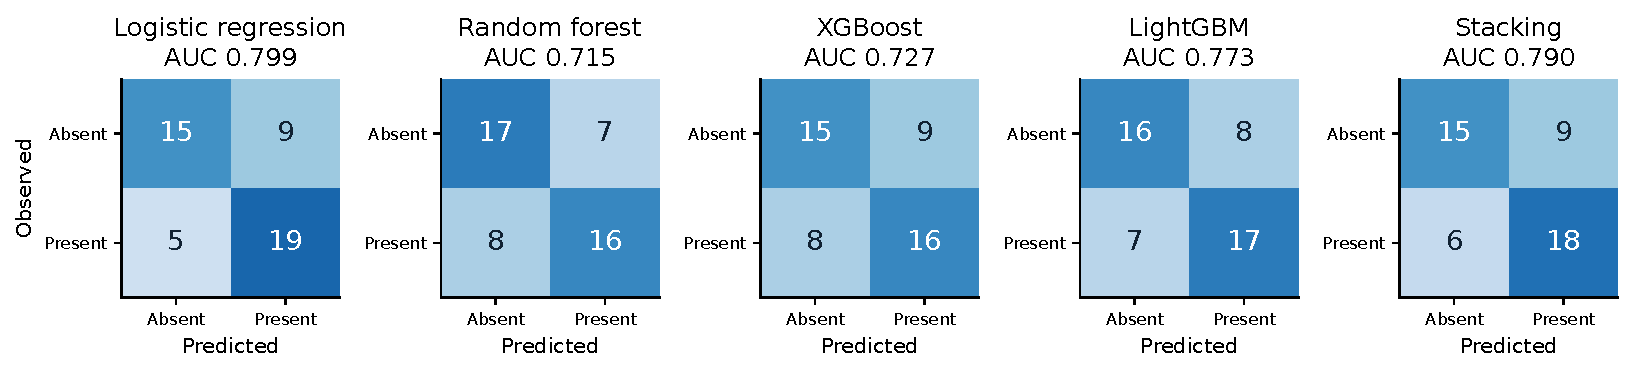
\includegraphics[width=\textwidth]{figures/modeling/execution_evidence.pdf}
\caption{Saved seed-42 validation outputs for all predictive families with
RFE--CART. Each confusion matrix contains 48 predictions at threshold 0.5;
class 1 denotes gallstones present. These are rendered numerical outputs,
not screenshots. Source: \protect\path{results/holdout/metrics.csv}.}
\label{fig:execution-evidence}
\end{figure}

\subsection{Statistical Patterns from the Fitted Models}
\label{subsec:statistical-patterns}
This section records numerical evidence. Interpretation is in
Section~\ref{subsec:pattern-discussion}, charts in
Section~\ref{subsec:pattern-visualisation}, and evaluation against the
project criteria in Section~\ref{subsec:model-evaluation}.

\paragraph{Holdout validation outputs.}
\label{subsec:python-building-selection}

Table~\ref{tab:building-validation-evidence} summarises the saved validation
results, not test rankings. Each cell reports mean $\pm$ sample variance
across five holdout seeds, using denominator $5-1$. This notation reports
variance, not standard deviation or a confidence interval. RFE denotes
RFE--CART; bold identifies the highest mean among predictive models in each
column, with the dummy shown separately as a benchmark.

\begin{table}[H]
\centering
\footnotesize
\setlength{\tabcolsep}{4pt}
\caption{Five-seed holdout validation: mean $\pm$ sample variance at threshold 0.5.}
\label{tab:building-validation-evidence}
\begin{tabular}{@{}lrrrr@{}}
\toprule
& \multicolumn{2}{c}{ROC--AUC} & \multicolumn{2}{c}{Sensitivity} \\
\cmidrule(lr){2-3}\cmidrule(l){4-5}
Model & CART & RFE & CART & RFE \\
\midrule
Logistic regression & $\mathbf{0.834 \pm 0.001306}$ & $\mathbf{0.838 \pm 0.001930}$ & $\mathbf{0.808 \pm 0.002257}$ & $\mathbf{0.758 \pm 0.002951}$ \\
Random forest       & $0.798 \pm 0.002135$ & $0.776 \pm 0.001504$ & $0.717 \pm 0.004688$ & $0.717 \pm 0.002083$ \\
XGBoost             & $0.791 \pm 0.001392$ & $0.777 \pm 0.001080$ & $0.742 \pm 0.003819$ & $0.708 \pm 0.000868$ \\
LightGBM            & $0.791 \pm 0.000612$ & $0.772 \pm 0.000973$ & $0.717 \pm 0.006424$ & $0.717 \pm 0.002083$ \\
Stacking            & $0.822 \pm 0.000825$ & $0.812 \pm 0.000558$ & $0.758 \pm 0.005556$ & $0.733 \pm 0.000521$ \\
\midrule
Training-prior dummy& $0.500 \pm 0.000000$ & $0.500 \pm 0.000000$ & $1.000 \pm 0.000000$ & $1.000 \pm 0.000000$ \\
\bottomrule
\end{tabular}
\end{table}

\paragraph{Leave-one-out outputs.}
\label{subsec:building-lopo-results}

Table~\ref{tab:building-lopo-results} reports the saved LOPO results from
\protect\path{results/lopo/metrics.csv}. Each model has 319 pooled held-out
predictions, using RFE--CART selection and seed 42. This is row-level LOOCV,
equivalent to leave-one-person-out only if each row is a different person.
There is one complete run, so no between-seed variance is reported. Bold marks
the highest predictive-model score in each column, except FNR, where lower
is better. These are complementary evaluation results, not a new basis for
overriding the validation-selected model family.

\begin{table}[H]
\centering
\small
\caption{LOPO evaluation on 319 held-out predictions per model at threshold 0.5.}
\label{tab:building-lopo-results}
\begin{tabular}{@{}lrrrrrr@{}}
\toprule
Model & Accuracy & ROC--AUC & Sensitivity & Specificity & F1 & FNR \\
\midrule
Logistic regression & 0.784 & \textbf{0.874} & 0.820 & 0.747 & 0.793 & 0.180 \\
Random forest & \textbf{0.799} & 0.857 & \textbf{0.839} & 0.759 & \textbf{0.808} & \textbf{0.161} \\
XGBoost & 0.762 & 0.835 & 0.807 & 0.715 & 0.774 & 0.193 \\
LightGBM & 0.787 & 0.851 & 0.832 & 0.741 & 0.798 & 0.168 \\
Stacking & 0.787 & 0.865 & 0.801 & \textbf{0.772} & 0.791 & 0.199 \\
\midrule
Training-prior dummy & 0.505 & 0.000 & 1.000 & 0.000 & 0.671 & 0.000 \\
\bottomrule
\end{tabular}
\end{table}


\paragraph{Numerical comparison of holdout and LOPO.}
The comparison fixes the algorithm settings and RFE--CART selector, avoiding
confounding evaluation method with CART versus RFE selection. Holdout test
entries describe every fixed candidate for comparison; they are not the
validation-selected procedure reported in Section~\ref{subsec:model-evaluation}.
Sources are \path{results/holdout/metrics.csv} and
\path{results/lopo/metrics.csv}. Interpretation and differences between the
evaluation designs are discussed in Section~\ref{par:holdout-lopo-discussion}.
\begin{table}[H]
\centering\small
\caption{Holdout and LOPO comparison for fixed RFE--CART candidates at threshold 0.5. Holdout entries average five seeds; LOPO entries pool 319 held-out predictions from one complete run.}
\label{tab:holdout-lopo-comparison}
\begin{tabular}{@{}lrrrrrr@{}}
\toprule
& \multicolumn{3}{c}{ROC--AUC} & \multicolumn{3}{c}{Sensitivity} \\
\cmidrule(lr){2-4}\cmidrule(l){5-7}
Model & Holdout val. & Holdout test & LOPO & Holdout val. & Holdout test & LOPO \\
\midrule
Logistic regression & 0.838 & 0.887 & 0.874 & 0.758 & 0.858 & 0.820 \\
Random forest & 0.776 & 0.850 & 0.857 & 0.717 & 0.850 & 0.839 \\
XGBoost & 0.777 & 0.844 & 0.835 & 0.708 & 0.858 & 0.807 \\
LightGBM & 0.772 & 0.841 & 0.851 & 0.717 & 0.850 & 0.832 \\
Stacking & 0.812 & 0.881 & 0.865 & 0.733 & 0.858 & 0.801 \\
\bottomrule
\end{tabular}
\end{table}


\paragraph{Conditional associations and extracted rules.}
Across five 20-feature RFE logistic fits, CRP, vitamin D, ECF/TBW and
haemoglobin were always selected, with mean transformed-scale coefficients
$-1.318$, $+0.690$, $+0.810$ and $+0.549$, respectively. Their mean validation
permutation AUC decreases were 0.1127, 0.0437, 0.0597 and 0.0172.
CRP was the root of all five direct CART selection trees: its recorded-scale
cut-point was 0.79 for seed 42 and 0.585 for the other four seeds.
The following counts describe seed-42 training nodes, not held-out risks.
\begin{table}[htbp]
\centering
\small
\caption{Conditional profiles extracted from the seed-42 CART selection tree.}
\label{tab:clinical-tree-patterns}
\begin{tabularx}{\textwidth}{Xrr}
\toprule
Model-defined subgroup & Present / total & Present (\%) \\
\midrule
CRP $\leq0.79$ & 100/138 & 72.5 \\
CRP $>0.79$ & 13/85 & 15.3 \\
CRP $\leq0.79$, total-body-fat ratio $\leq32.1$ & 87/107 & 81.3 \\
CRP $\leq0.79$, total-body-fat ratio $>32.1$ & 13/31 & 41.9 \\
CRP $>0.79$, vitamin D $\leq22.5$ & 3/60 & 5.0 \\
CRP $>0.79$, vitamin D $>22.5$ & 10/25 & 40.0 \\
\bottomrule
\end{tabularx}
\end{table}